\documentclass[10pt]{article}
\usepackage[utf8]{inputenc}
\usepackage[T1]{fontenc}
\usepackage{graphicx}
\usepackage[export]{adjustbox}
\graphicspath{ {./images/} }
\usepackage{amsmath}
\usepackage{amsfonts}
\usepackage{amssymb}
\usepackage[version=4]{mhchem}
\usepackage{stmaryrd}

\begin{document}
\begin{center}
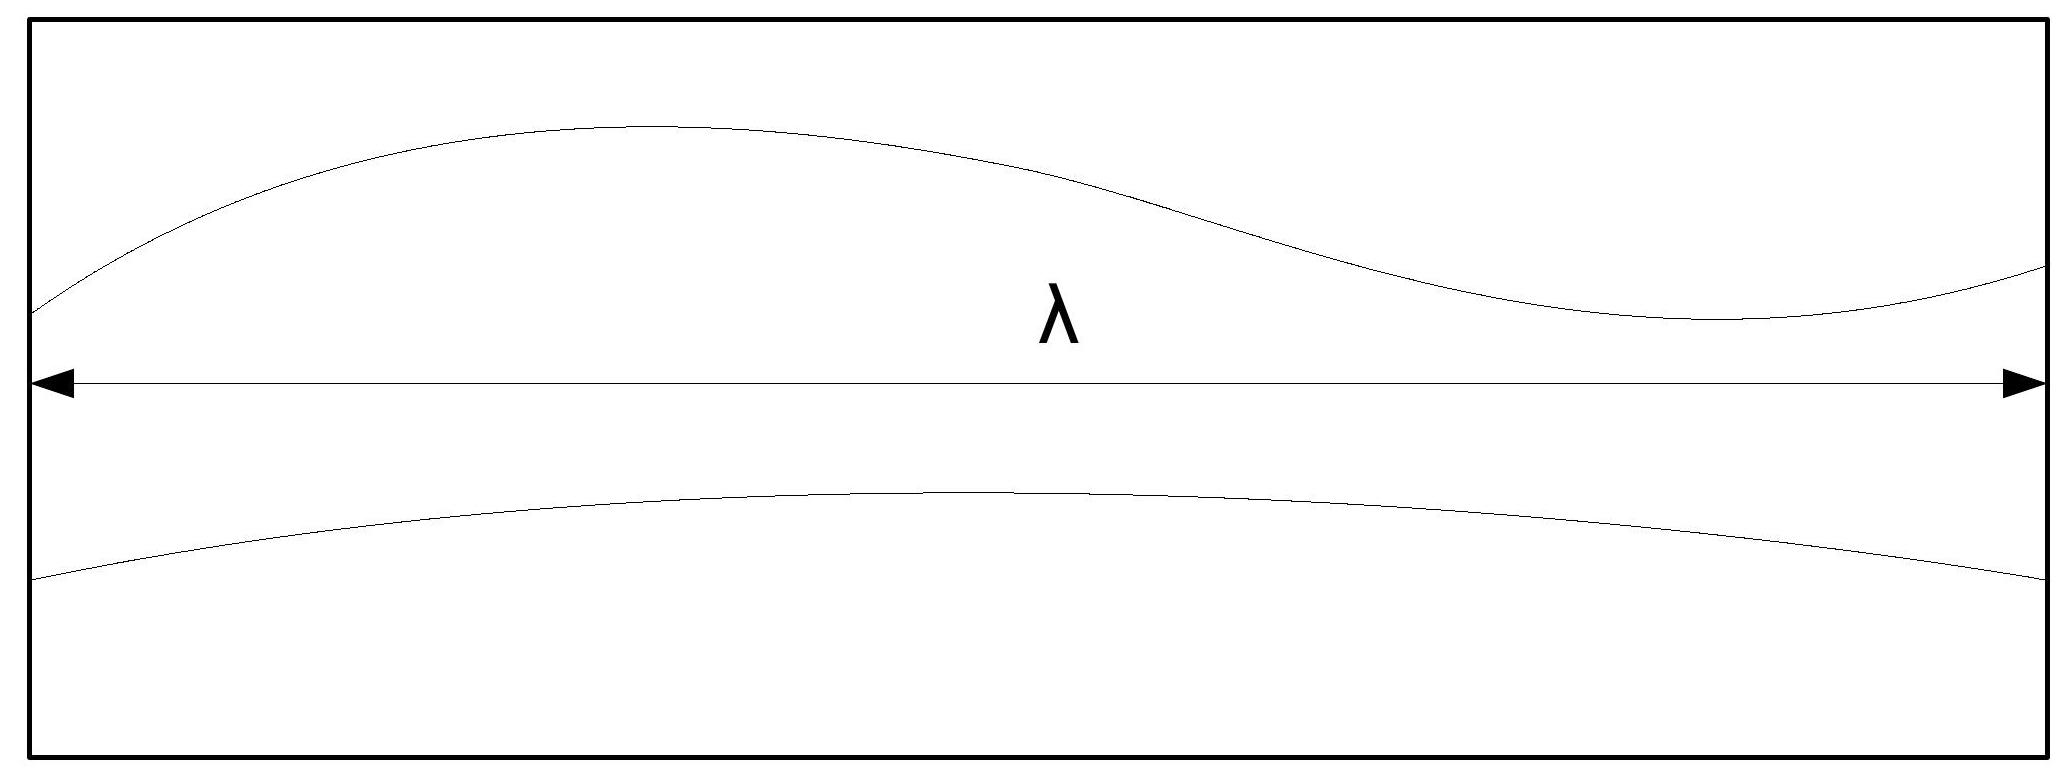
\includegraphics[max width=\textwidth]{2023_05_21_66a3dfca5be088b7d6b7g-01}
\end{center}

В результате энергетический спектр становится дискретным

$$
U(x, y, z)=\left\{\begin{array}{cc}
0, & 0 \leq z \leq L_{z} \\
U_{0,} & z<0, z>L_{z}
\end{array}\right\}
$$

\begin{center}
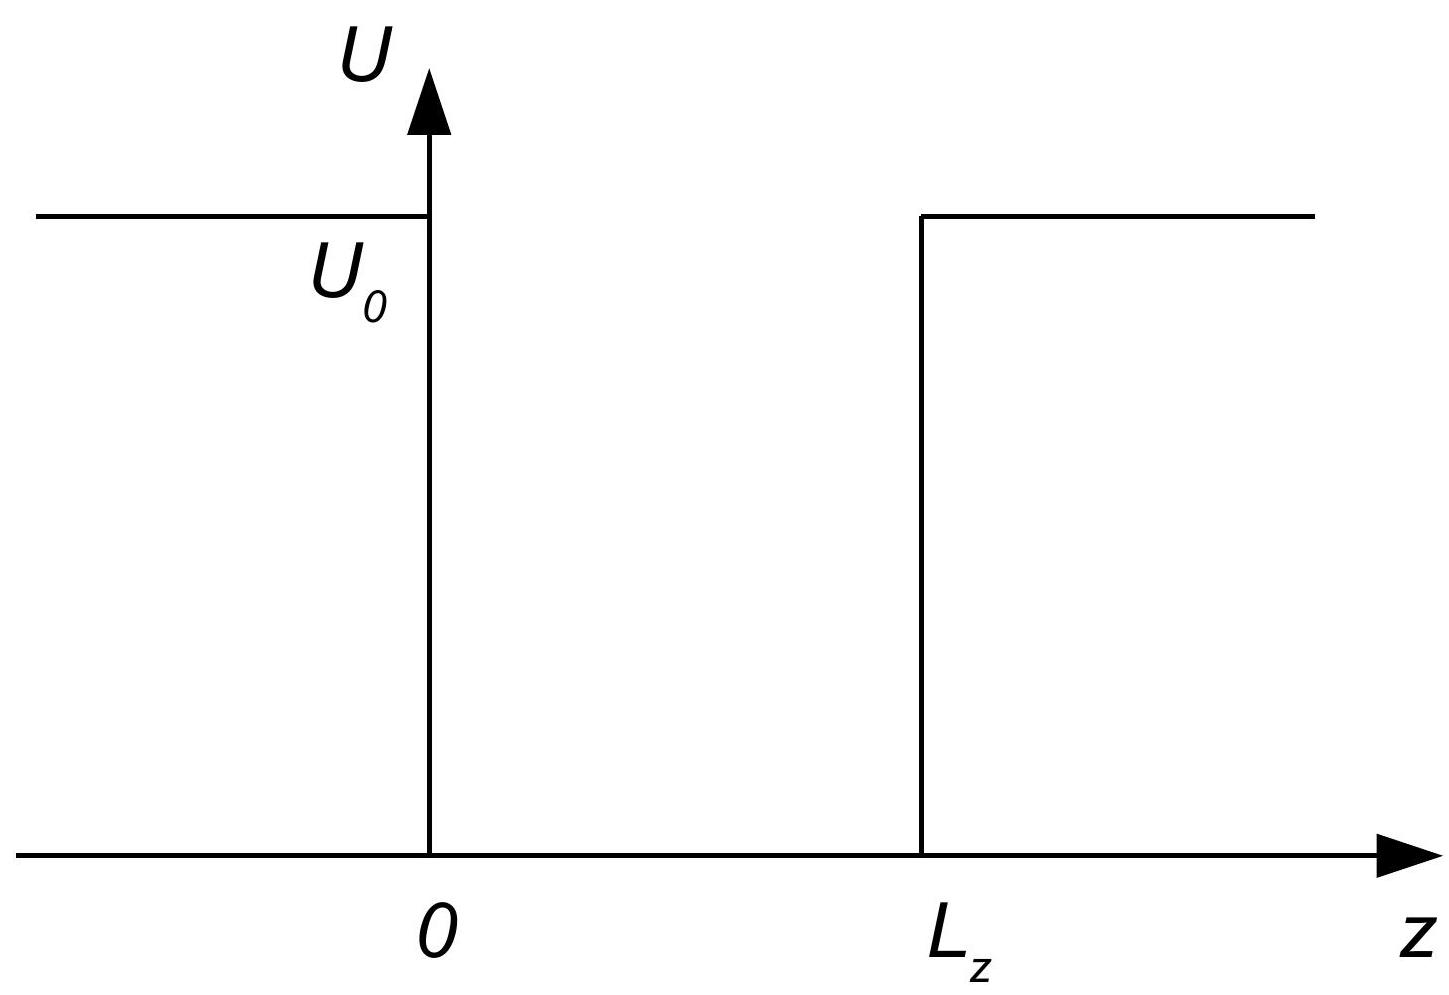
\includegraphics[max width=\textwidth]{2023_05_21_66a3dfca5be088b7d6b7g-02}
\end{center}

Нет зависимости потенциальной энергии от х, у в явном виде, поэтому:

$$
\psi(x, y, z)=\exp \left(i\left(k_{x} x+k_{y} y\right)\right) \psi_{z}(z)
$$

$k_{x}, k_{y}$ - компоненты волнового вектора вдоль $\mathrm{x}, \mathrm{y}$

\section{Оператор Гамильтона и уравнение Шредигера}
$$
\begin{aligned}
\hat{H}= & -\frac{\hbar^{2}}{2 m_{e}}\left(\frac{\partial^{2}}{\partial x^{2}}+\frac{\partial^{2}}{\partial y^{2}}+\frac{\partial^{2}}{\partial z^{2}}\right)+U(x, y, z) \\
& \hat{H} \psi(x, y, z)=E \psi(x, y, z)
\end{aligned}
$$

Подстановка волновой функции в уравнение даёт

$$
\frac{d^{2} \psi_{z}}{d z^{2}}+\frac{2 m_{e}}{\hbar^{2}}\left(E-\frac{\hbar^{2}}{2 m}\left(k_{x}^{2}+k_{y}^{2}\right)-U(z)\right) \psi_{z}=0
$$

$$
U_{0} \rightarrow \infty
$$

Волновая функция должна быть равна нулю в области с бесконечной потенциальной энергией:

$$
\psi_{z}=\left\{\begin{array}{c}
c_{m s} \sin \left(k_{z} z\right)+c_{m c} \cos \left(k_{z} z\right), \quad 0 \leq z \leq L_{z} \\
0, \quad z<0, z>L_{z}
\end{array}\right.
$$

Граничное условие при z=0 даёт $c_{m c}=0$. Граничное условие при $z=L_{z}$ даёт:

$$
k_{z}=\frac{\pi n}{L_{z}}, n=1,2,3 \ldots
$$

Условие нормировки даёт: $\quad c_{m s}=\sqrt{\frac{2}{L_{z}}}$ Потенциальный ящик с бесконечными стенками. Решения.

$$
\begin{gathered}
\psi_{z}=\left\{\begin{array}{c}
\sqrt{\frac{2}{L_{z}}} \sin \left(\frac{\pi n z}{L_{z}}\right), \quad 0 \leq z \leq L_{z} \\
0, z<0, z>L_{z}
\end{array}\right. \\
E-\frac{\hbar^{2}}{2 m_{e}}\left(k_{x}^{2}+k_{y}^{2}\right)=\frac{\hbar^{2} k_{z}^{2}}{2 m_{e}} \quad E=\frac{\hbar^{2}}{2 m_{e}}\left(k_{x}^{2}+k_{y}^{2}\right)+\frac{\pi^{2} \hbar^{2} n^{2}}{2 m_{e} L_{z}^{2}}, n=1,2,3 \ldots
\end{gathered}
$$

\begin{center}
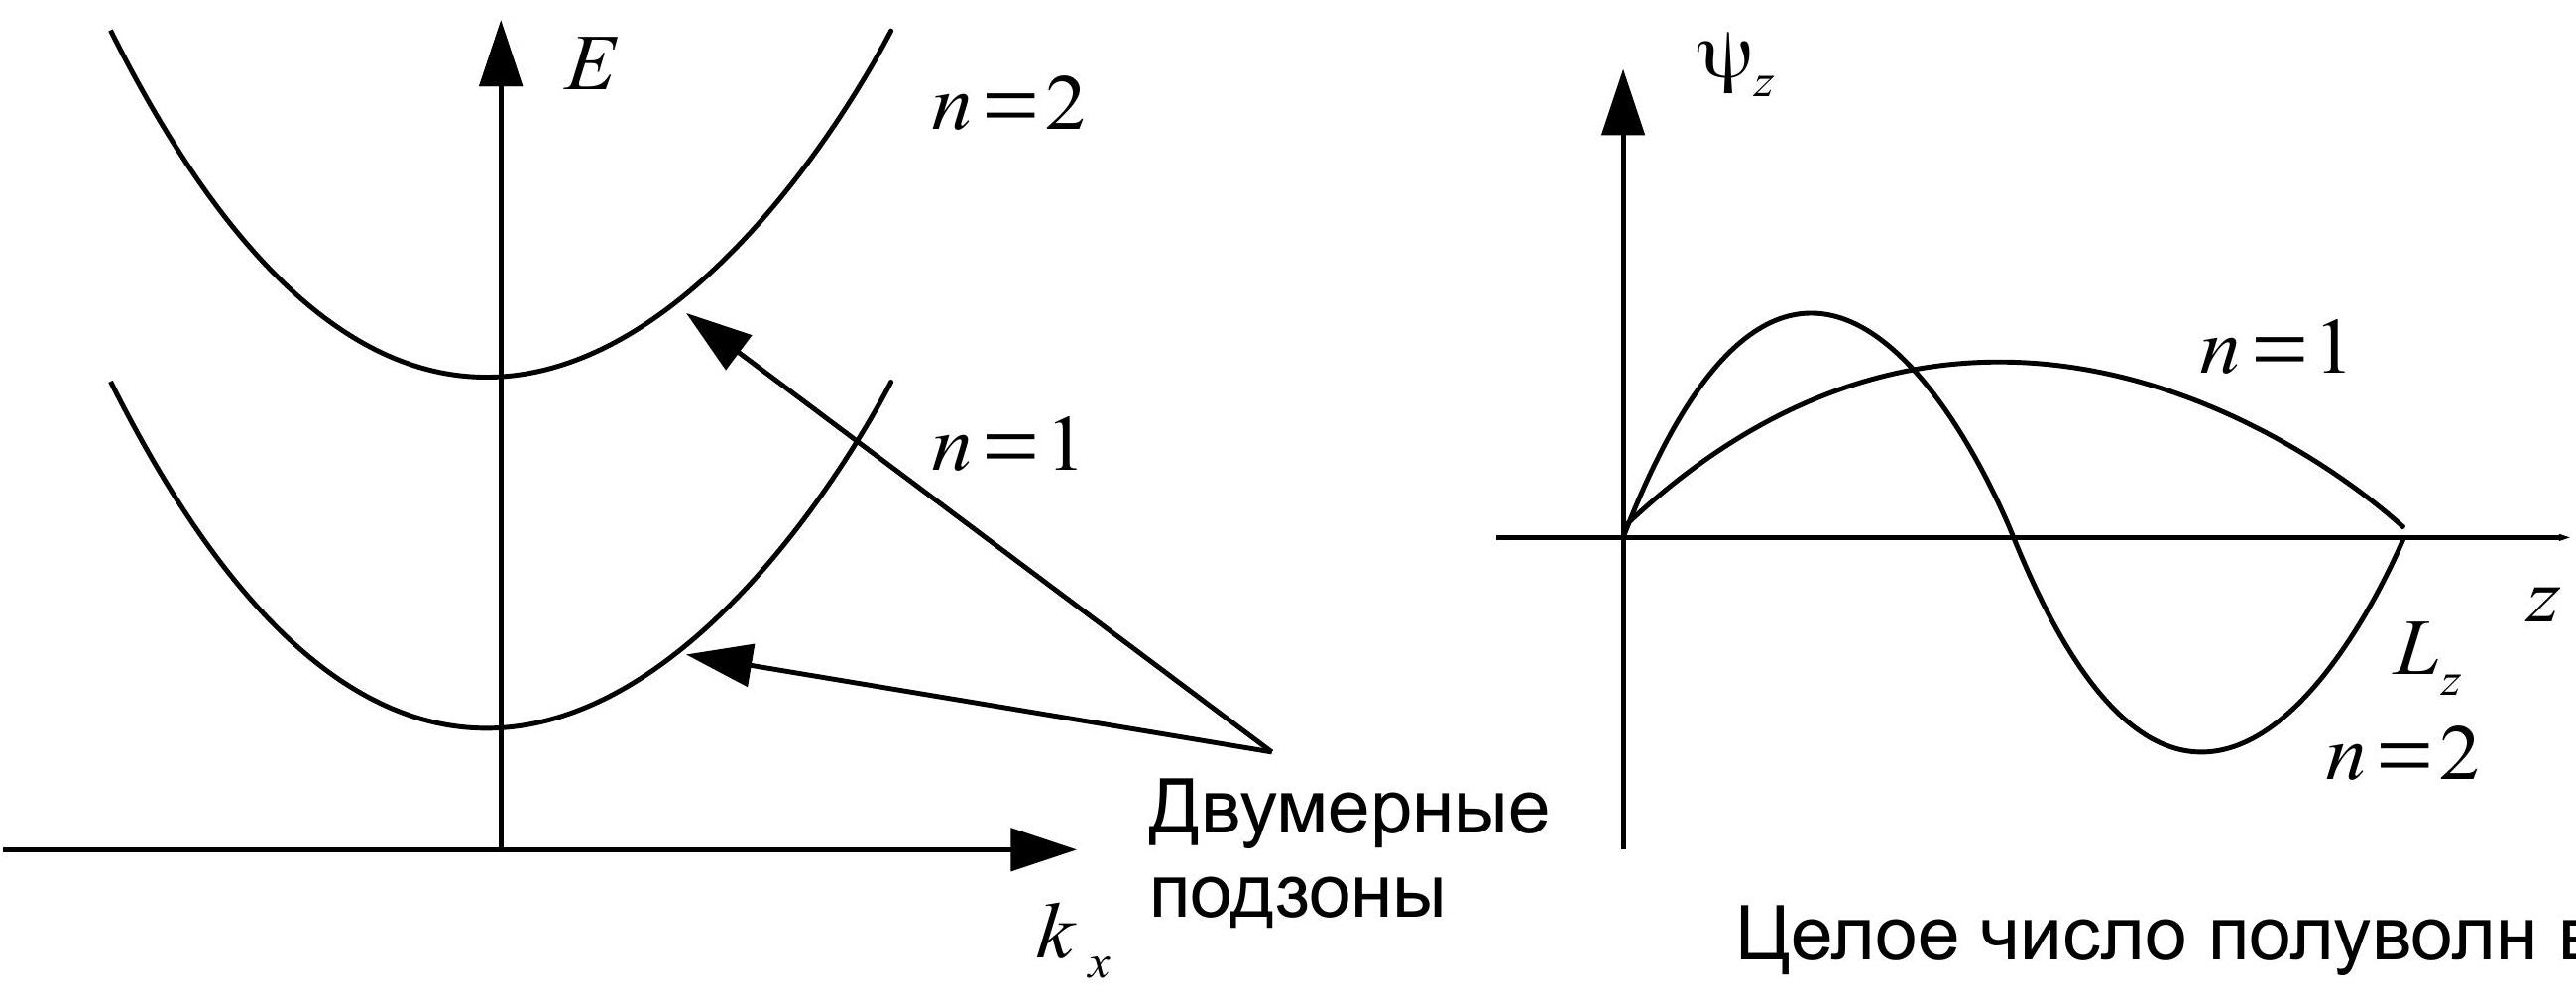
\includegraphics[max width=\textwidth]{2023_05_21_66a3dfca5be088b7d6b7g-05}
\end{center}

Целое число полуволн в структуре

\section{Решения внутри ящика $E<U_{0}$}
$$
\psi_{z}=\left\{\begin{array}{c}
c_{l} \exp \left(\frac{\sqrt{2 m\left(U_{0}-E\right)}}{\hbar} z\right), \quad z<0 \\
c_{m s} \sin \left(\frac{\sqrt{2 m E}}{\hbar} z\right)+c_{m c} \cos \left(\frac{\sqrt{2 m E}}{\hbar} z\right), 0 \leq z \leq L_{z} \\
c_{r} \exp \left(-\frac{\sqrt{2 m\left(U_{0}-E\right)}}{\hbar} z\right), \quad z>L_{z}
\end{array}\right\}
$$

Непрерывность волновой функции и её производной при z=0 и z= $L_{z}$ даёт систему линейных однородных уравнений относительно коэфициентов $c$ :

$$
\begin{gathered}
c_{l}=c_{m c} \\
c_{l} \sqrt{2 m \frac{\left(U_{0}-E\right)}{\hbar}}=c_{m s} \frac{\sqrt{2 m E}}{\hbar} \\
c_{m s} \sin \left(\frac{\sqrt{2 m E}}{\hbar} L_{z}\right)+c_{m c} \cos \left(\frac{\sqrt{2 m E}}{\hbar} L_{z}\right)=c_{r} \exp \left(-\frac{\sqrt{2 m\left(U_{0}-E\right)}}{\hbar} L_{z}\right) \\
c_{m s} \frac{\sqrt{2 m E}}{\hbar} \cos \left(\frac{\sqrt{2 m E}}{\hbar} L_{z}\right)-c_{m c} \frac{\sqrt{2 m E}}{\hbar} \sin \left(\frac{\sqrt{2 m E}}{\hbar} L_{z}\right)=-c_{r} \frac{\sqrt{2 m\left(U_{0}-E\right)}}{\hbar} \exp \left(-\frac{\sqrt{2 m\left(U_{0}-E\right)}}{\hbar} L_{z}\right)
\end{gathered}
$$

Ненулевые решения при определителе матрицы системы уравнений равном нулю. Это даёт уравнение на $E$, которое имеет несколько решений.

\section{При любом $E>U_{0}$ существует ненулевое решение незатухающее при}
 удалении от потенциального ящика (трёхмерного)\begin{center}
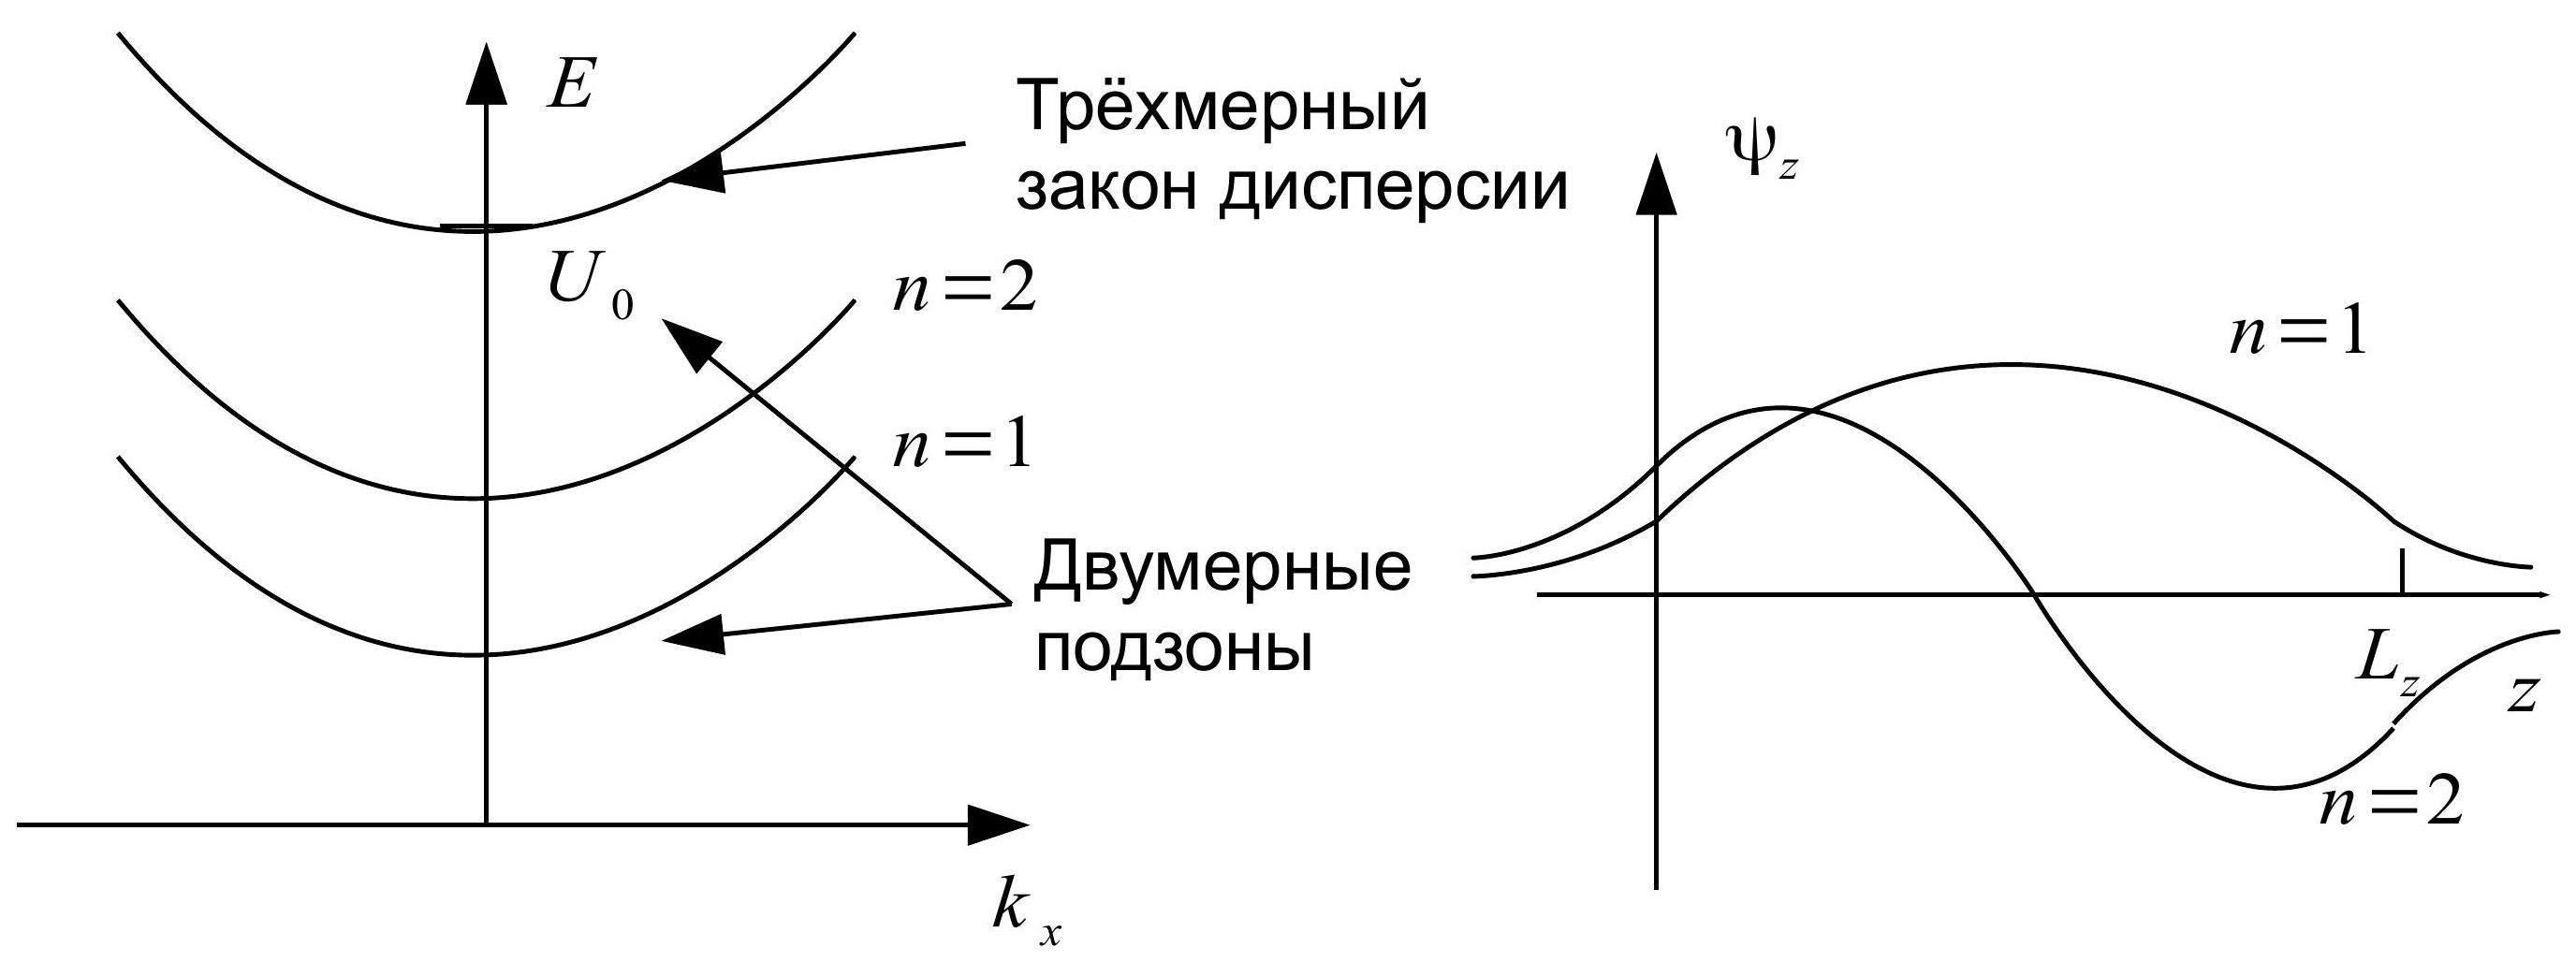
\includegraphics[max width=\textwidth]{2023_05_21_66a3dfca5be088b7d6b7g-07}
\end{center}

Волновые фукции двумерных состояний сосредоточены внутри потенциальной ямы для электронов дырок

В двумерной структуре образуется конечное число двумерных подзон.

При энергии выше потенциального барьера, ограничивающего потенциальную яму существуют трёхмерные состояния

При наличии потенциальной ямы для дырок образуются двумерные подзоны для дырок

Закон дисперсии вблизи минимума двумерной подзоны квадратичный, но может быть анизотропным при анизотропии материала структуры

$$
E=E_{n}+\frac{\hbar^{2}}{2}\left(\frac{k_{x}^{2}}{m_{x x}}+\frac{k_{y}^{2}}{m_{y y}}\right), n=1,2,3 \ldots
$$

При наличии двух типов посителей (например лёгкие и тяжёлые дырки) образуется набор двумерных подзон для носителей каждого типа Квантовая нить - одномерная структура, размеры которой в двух направлениях сопоставимы с длиной волны (длиной свободного пробега) электронов. В квантовых нитях проявляется эффрект размерного квантования.

Нанонить - структура, размеры которой в двух направлениях менее нескольких сотен нанометров. В нанонитях размерное квантование может не проявляться

\begin{center}
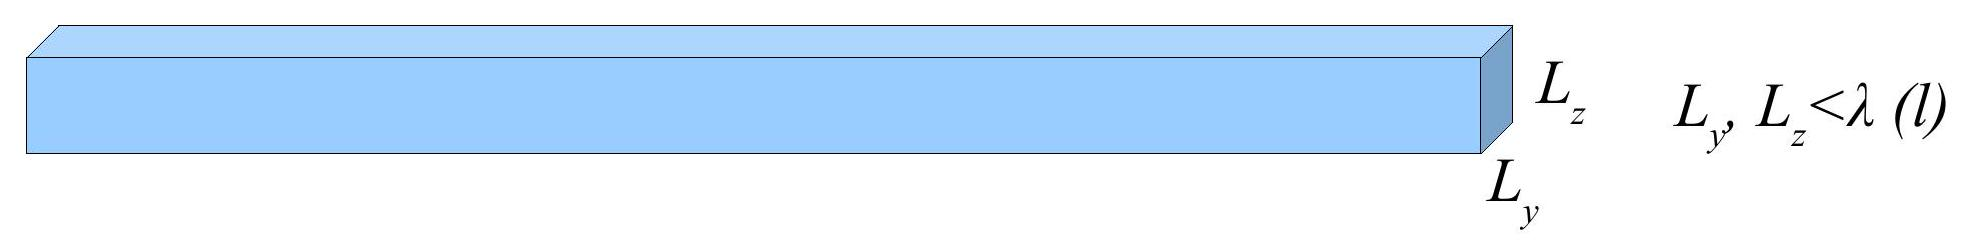
\includegraphics[max width=\textwidth]{2023_05_21_66a3dfca5be088b7d6b7g-09}
\end{center}

Квантовая точка - нульмерная структура, размеры которой в трёх направлениях сопоставимы с длиной волны (длиной свободного пробега) электронов. В квантовых точках проявляется размерное квантование

\begin{center}
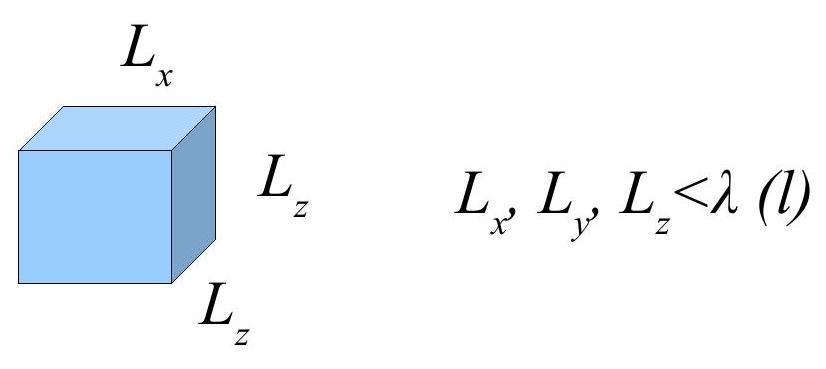
\includegraphics[max width=\textwidth]{2023_05_21_66a3dfca5be088b7d6b7g-09(1)}
\end{center}

Расчёт из первых принципов - исходит из состава и положения отдельных атомов (ab initio)

Приближённые методы: самосогласованное решение уравнений Шредингера (в приближении эффрективной массы или огибающей функции) и Пуассона с добавлением обменно-корреляционного потенциала. Исходные данные - макроскопические свойства материалов слоёв структуры

\section{Квадратичный закон дисперсии}
$$
E(\vec{k})=E_{n}+\frac{\hbar^{2}}{2}\left(\frac{k_{x}^{2}}{m_{x}}+\frac{k_{y}^{2}}{m_{y}}\right)
$$

Плотность состояний

$$
v_{2 D}(E)=\frac{\partial N_{2 D}\left(E^{\prime}<E\right)}{\partial E}
$$

$N_{2 \mathrm{D}}\left(E^{\prime}<E\right)$ - концентрация (на единицу площади) состояний с энергией $E^{\prime}<E$

$$
N_{2 D}\left(E^{\prime}<E\right)=\frac{2}{(2 \pi)^{2}} \sum_{n} S_{n}(E<E)=\frac{2 \cdot 2 \pi \sqrt{\left(m_{x} m_{y}\right)} E}{4 \pi^{2} \hbar^{2}} \sum_{n} \theta\left(E-E_{n}\right)
$$

\section{$S_{n}\left(E^{\prime}<E\right)$ - площадь состояний в простансте квазиволновых векторов, занимаяемая состояниями с энергией $E^{\prime}<E$ в $n$-ой двумерной подзоне}
$$
\theta(x)=\left\{\begin{array}{l}
1, x \geq 0 \\
0, x<0
\end{array}\right.
$$

$$
v_{2 D}=\sum_{n} \frac{\sqrt{m_{x} m_{y}}}{\pi \hbar^{2}} \theta\left(E-E_{n}\right)
$$

\begin{center}
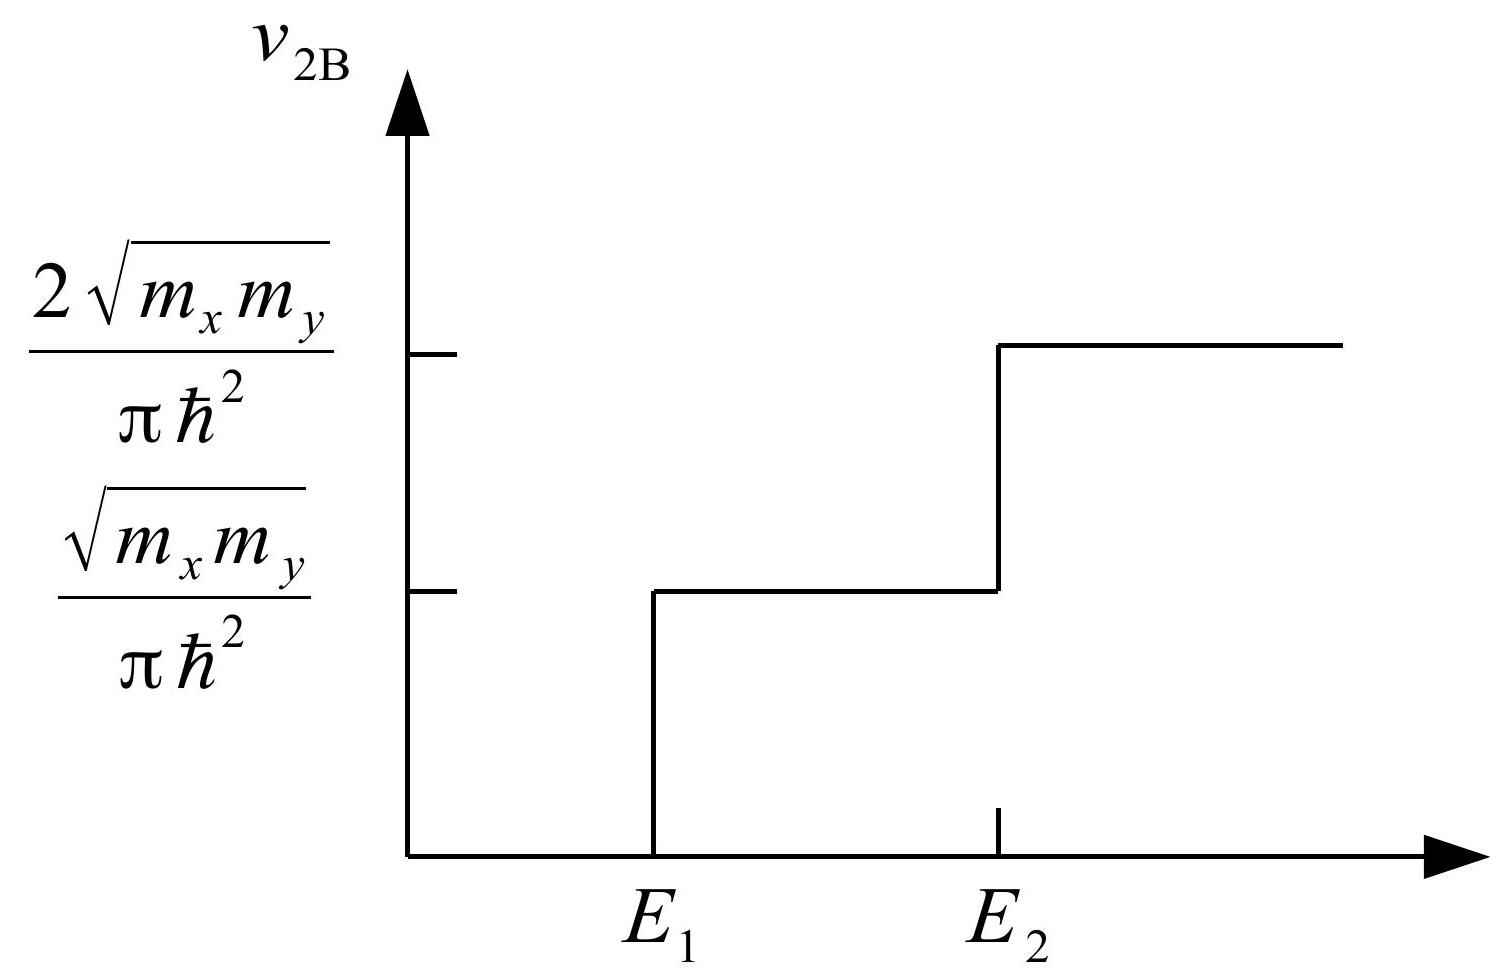
\includegraphics[max width=\textwidth]{2023_05_21_66a3dfca5be088b7d6b7g-12}
\end{center}

Концентрация двумерных электронов

$$
n_{2 \mathrm{D}}=\int_{-\infty}^{\infty} v_{2 \mathrm{D}}(E) f(E) d E
$$

При $T=0$ (квадратичный закон дисперсии):

$$
n_{2 D}=\sum_{n} \frac{\sqrt{m_{x} m_{y}}}{\pi \hbar^{2}}\left(F-E_{n}\right) \theta\left(F-E_{n}\right)
$$

При T>0 (квадратичный закон дисперсии):

$$
\begin{aligned}
& f(E)=\frac{1}{\exp \left(\frac{E-F}{k_{B} T}\right)+1} \\
& n_{2 D}=\sum_{n} k_{B} T \frac{\sqrt{m_{x} m_{y}}}{\pi \hbar^{2}} \ln \left(1+\exp \left(\frac{F-E_{n}}{k_{B} T}\right)\right)
\end{aligned}
$$


\end{document}